{\bf \huge Part I:}
\vspace{0.7cm}
 
{\bf \Huge Installation and Setup }

\vspace{0.5cm}

This part provides a very simple example and a JUnit test to check the installation and configuration of eMoflon. It can be considered \emph{mandatory} if you
are new to eMoflon, but we recommend working through it anyway.

After working through this part, you should have an installed and tested eMoflon working for a trivial example. We also explain the general workflow, the
different workspaces involved.

\requiredTime{Just a few minutes\ldots}

\downloadLocation{\dlPartOne}

% Welcome Summary
\section{Getting started}
\genHeader 

Here's how we've organized our handbooks; Black, red, and blue headers are used to separate common, visual, and textual syntax
instructions (Fig~\ref{pageExamples}).

\begin{figure}[htbp] \centering
  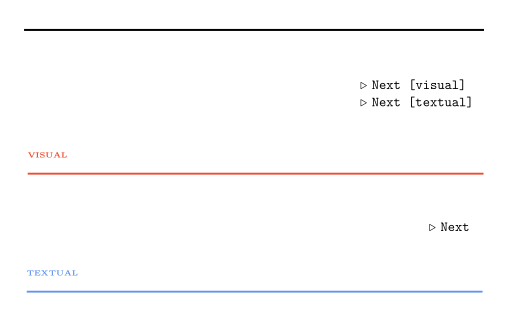
\includegraphics[width=0.9\textwidth]{headers}
	\caption{Page headers and links}
	\label{pageExamples} 
\end{figure}

You'll find a \mbox{ $\triangleright$ {\texttt{link}} } at the bottom of some pages. These will take you to the next appropriate place for your syntax.
You are still welcome to go through the entire handbook page by page. In fact, we encourage it and hope you'll compare the differences and similarities
between the two specifications. But be warned! If what you're doing isn't matching what you see, you may be reading the wrong instructions.

If, however, you're finding that the screenshots we've taken aren't matching your screen and you ARE in the right place, please send us an email at
\href{mailto:contact@moflon.org}{contact@moflon.org} and let us know. They get outdated so fast! They just grow up, move on, start doing their own thing and
\ldots uh, wait a second. We're talking about pictures here.

Here are some guidelines to help you decide which syntax to use:

\begin{itemize}

\item[$\blacktriangleright$] If you have used a UML tool before and feel comfortable with the standard UML diagrams, then you might prefer our visual syntax.

\item[$\blacktriangleright$] If you do not like switching tools, and want everything integrated completely in Eclipse with zero installation, then you should stick to our textual syntax.

\item[$\blacktriangleright$] If you use a Mac (or some other *Nix system) then you will need virtualisation software to run Windows and install the required UML
tool for our visual syntax. Most maconians find this insulting and of course choose our textual syntax.

\item[$\blacktriangleright$] As a final remark, consider that graph transformations obviously have something to do with graphs, which are inherently two dimensional structures. 
A visual syntax thus has some obvious advantages and is what we (currently) prefer and use internally (eMoflon is built with eMoflon).

\end{itemize}


% Common instructions
\genHeader
\fancyfoot[RE]{ $\triangleright$ \hyperlink{installEA vis}{Next visual task} \\ $\triangleright$ \hyperlink{simpleDemo common}{Next textual step} }

\section{Install our plugin for Eclipse}
 
 \vspace{0.5cm}
 
\begin{itemize}
\item[$\blacktriangleright$] Download and install Eclipse for Modelling ``Eclipse Modeling Tools (includes incubating components)''\footnote{Please note that you \emph{have to} install \emph{Eclipse Modeling Tools}, from the Juno download packages, or nothing will work.  Do not choose a different Eclipse package!  Although different versions might work, eMoflon is currently tested for Eclipse Juno and Java 1.7.} from \url{http://www.eclipse.org/downloads/packages/release/juno/sr2} (Fig.~\ref{fig_downloadModelingPackage}).

\vspace{1.5cm}

\begin{figure}[htbp]
	\centering
  	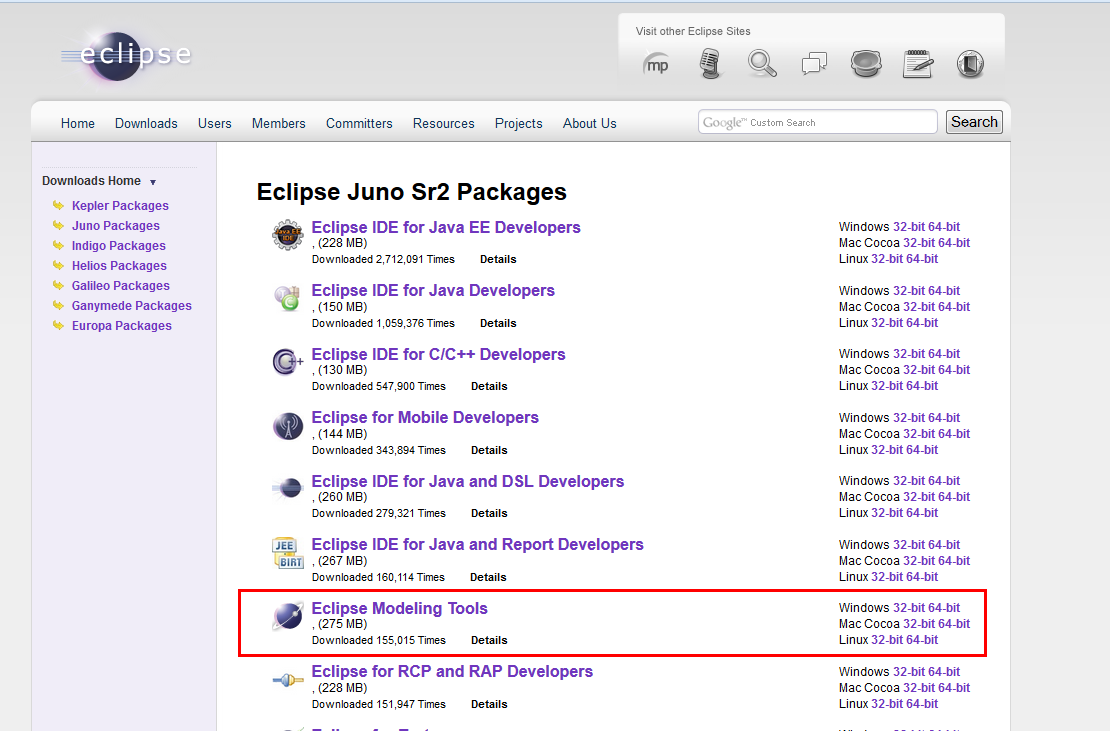
\includegraphics[width=0.86\textwidth]{eclipse_modelingTools}
	\caption{Download Eclipse Modeling Tools.}
	\label{fig_downloadModelingPackage}
\end{figure}

\vspace{1cm}

\item[$\blacktriangleright$] Install our Eclipse Plugin from the following update site\footnote{For a detailed tutorial on how to install Eclipse and Eclipse Plugins please refer to \url{http://www.vogella.de/articles/Eclipse/article.html}} 
\footnote{Please note: Calculating requirements and dependencies when installing the plugin might take quite a while depending on your internet connection.}:
\url{http://www.moflon.org/fileadmin/download/moflon-ide/eclipse-plugin/update-site2}

\end{itemize}


% Visual instructions; install EA
% -----------------------------------------------------------------------------------------------------------------------------------
% -------- VISUAL -------------------------------------------------------------------------------------------------------------------
\newpage

\section{Install our extension for Enterprise Architect}

\newpage
\texHeader
\mbox{}

\newpage
\texHeader
\mbox{}
